% ------------------------
% Declaração do documento |
% ------------------------
\documentclass{article}
% ----------------------------
% Pacotes usados no documento |
% ----------------------------
\usepackage[utf8]{inputenc}
\usepackage[left=2cm,top=2cm,right=3cm,bottom=3cm]{geometry}
\usepackage[ampersand]{easylist}
\usepackage{graphicx}
\usepackage{enumitem}

% --------------------
% Inicio do documento |
% --------------------
\begin{document}
\par Nome: Pablo Emanuell Lopes Targino
\par Matricula: 20170067995 \bigskip \bigskip

	Para a desenhar as interfaces utilizei o software Balsamiq.
	
	A ideia consiste em projetar um aplicativo de divulgação de eventos e novos estabelecimentos, por meio de cadastros feitos pelo usuário.
	Quando o usuário assumi o papel de divulgador de eventos, suas atribuições são:\medskip
	\begin{easylist}[itemize]
	& Divulgar um evento.
	& Gerenciar seus eventos.
	& Ver histórico de eventos realizados por ele.
	\end{easylist}\medskip
	Ao divulgar um evento o usuário deve fornecer o nome do evento, o horário, a localização, uma imagem do evento, uma indicação se o evento é público ou privado e, opcionalmente, observações sobre o evento. A tela que ele usurá para fazer isso será parecida com essa:
	% colocar tela
	\bigskip
	
	\begin{center}
	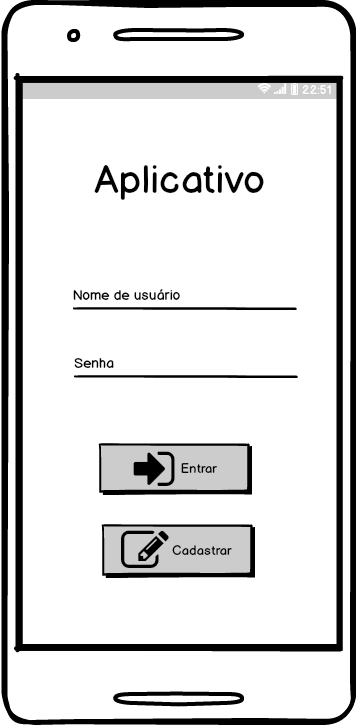
\includegraphics[scale=0.25]{ECV.png}
	\end{center}
	
	\bigskip
	Ao ao final do procedimento o evento estará disponível para que os outros usuários que tenham acesso a ele vejam e possam sinalizar sua participação.  
	
	Uma vez divulgado o evento poderá ser gerenciado. As operações possíveis relativas a essa possibilidade serão discutidas no decorrer do desenvolvimento do projeto.  
	
	O histórico de eventos realizados pelo divulgador estará disponível ao divulgar seu primeiro evento. Ao acessar esse menu, o usuário poderá ver todas as informações do eventos que já realizou. A tela onde as duas últimas operações serão realizadas será um menu drop-down que será apresentado junto com as operações do papel a seguir.
	
	Os eventos divulgados no sistema serão usados por pessoas que estão procurando lugares para sair, nesse papel as atribuições do usuário serão as seguintes:\medskip
	\begin{easylist}[itemize]
	& Ver eventos disponíveis na região.
	& Favoritar categorias de evento.
	& Ver agenda de eventos.
	& Ver histórico de eventos.
	\end{easylist}\medskip
	
	Para ver os eventos o usuário se utilizará de um mapa com coordenadas pré-configuradas para seu local (ou para o evento mais próximo). Os pontos no mapa, possivelmente, terão a mesmo tamanho, pois não queremos que um evento seja mais chamativo que outro, porém ainda será discutido como irão aparecer os eventos de categorias marcadas como favorita ou normal. O protótipo de tela para essa funcionalidade se encontra abaixo:
	% colocar tela
	As categorias favoritas vão servir para cada usuário ser notificado de eventos recentes que eles poderiam gostar. Na aba principal ele poderá ver todas as categorias e marcar as que ele mais gosta, como pode ser visto na imagem: 
	% colocar tela
	Como o aplicativos é de eventos, em geral é natural que o usuário queira ter alguma maneira de se lembrar de onde tem que ir. Para isso iremos dispor de uma agenda que conterá as datas do eventos que ele marcou presença. Além disso um aplicativo irá disparar uma notificação em determinado tem antes do evento. A tela será baseado no protótipo abaixo:
	% colocar tela
	Também é comum que uma pessoa queira se lembrar de onde ela foi determinado dia, essa funcionalidade estará disponível no sistema. A imagem abaixo demonstra como isso será feito.
	% colocar tela 
	 
	\section{Casos de uso} 
	\noindent\fbox{
		\parbox{\textwidth}{
			\begin{center}
				{\large \textbf{Divulgar evento (CSU01)}}
			\end{center}
	
			\textbf{Sumário:} Usuário cadastra um novo evento ao sistema.\medskip		
			
			\textbf{Ator Primário:} Divulgador\medskip	
		
			\textbf{Precondições:} Usuário está autentificado.\medskip
			
			\textbf{Fluxo Principal:}
			\begin{enumerate}[itemsep=0mm]
			 \item Usuário solicita o cadastro de um novo evento.
			 \item Sistema exibe formulário de cadastramento.
			 \item Usuário fornece os dados necessário.
			 \item Sistema cadastra novo evento e o caso de uso termina.
			\end{enumerate}
		}
	}\bigskip
	
	Gerenciar eventos (CSU02)
	
	Sumário: Usuário consultar eventos criados por ele.
	
	Ator Primário: Divulgador.
	
	Precondições: Usuário está autentificado e já criou no mínimo um evento.
	
	Fluxo Principal:
	
	1. Usuário solicita ao sistema eventos criados por ele.
	
	2. Sistema exibi uma lista de eventos cadastrados pelo usuário.
	
	3. Usuário seleciona um dos eventos.
	
	4. Sistema exibe as informações sobre o evento.
	
	5. Usuário cancela o evento ou edita as informações e o caso de uso termina.\bigskip
	
	Ver histórico de eventos (CSU03)
	
	Sumário: Usuário acessa informações sobre eventos que ele realizou.
	
	Ator Primário: Divulgador
	
	Precondições: Usuário está autentificado e já criou no mínimo um evento.
	
	Fluxo Principal:
	
	1. Usuário solicita ao sistema eventos já realizados por ele.
	
	2. Sistema exibi lista de eventos.
	
	3. Usuário seleciona um dos eventos.
	
	4. Sistema exibe as informações sobre o evento.
	
	5. Usuário visualiza as informações e o caso de uso termina.\bigskip
	
	Participar de  eventos (CSU04)
	
	Sumário: Usuário visualiza eventos próximos a ele.
	
	Ator Primário: Usuário procurando eventos.
	
	Precondições: Usuário está autentificado e existem eventos próximos a ele.
	
	Fluxo Principal:
	
	1. Usuário solicita eventos na proximidade.
	
	2. Sistema exibe os eventos próximos.
	
	3. Usuário escolhe um dos eventos.
	
	4. Sistema exibe informações sobre o evento.
	
	5. Usuário decide se vai participar do evento.
	
	6. Sistema cadastra participação no evento, se o usuário desejar, e o caso de uso termina.\bigskip
	
	Ver agenda(CSU05)
	
	Sumário: Usuário visualiza agenda mensal com eventos marcados.
	
	Ator Primário: Usuário procurando eventos.
	
	Precondições: Usuário está autentificado.
	
	Fluxo Principal:
	
	1. Usuário solicita eventos marcados com participação.
	
	2. Sistema exibe calendário com datas de participação em um evento.
	
	3. Usuário seleciona um data.
	
	4. Sistema exibi lista com eventos que o usuário participa.
	
	5. Usuário visualiza os eventos e o caso de uso termina.
	
	 (CSU01)
	
	Sumário: 
	
	Ator Primário: 
	
	Precondições: 
	
	Fluxo Principal:
	
	 (CSU01)
	
	Sumário: 
	
	Ator Primário: 
	
	Precondições: 
	
	Fluxo Principal:
	
	
	
	 

	
	


\begin{easylist}[articletoc]
\end{easylist}
\end{document}
% TODO: Fazer CSU04 